\documentclass[a4paper, 10pt]{article}    
\usepackage{geometry}       
\geometry{a4paper}
\geometry{margin=1in} 
\usepackage{paralist}
  \let\itemize\compactitem
  \let\enditemize\endcompactitem
  \let\enumerate\compactenum
  \let\endenumerate\endcompactenum
  \let\description\compactdesc
  \let\enddescription\endcompactdesc
  \pltopsep=\medskipamount
  \plitemsep=1pt
  \plparsep=1pt
\usepackage[english]{babel}
\usepackage[utf8]{inputenc}

\usepackage{bbm, bm}
\usepackage{amsmath, amssymb, amsthm, mathrsfs}
\usepackage{booktabs, tikz}

\pagestyle{headings}
\newcommand{\boxwidth}{430pt}

\theoremstyle{definition}
\newtheorem{problem}{Problem}

\newtheoremstyle{hSol}
  {1.0pt}% Space above
  {1.0pt}% Space below
  {}% bodyfont
  {}% indent
  {\bfseries}% thm head font
  {.}% punctuation after thm head
  { }% Space after thm head
  {}% thm head spec

\theoremstyle{hSol}
\newtheorem*{solution}{Solution}



\title{\textbf{Numerical Solutions for DEs HW3}}
\author{YANG, Ze (5131209043)}


\begin{document}
\maketitle


%------------------------------------------------------------------------
~\\
\fbox{
  \parbox{\boxwidth}{
  \textbf{A Note to TA}: 
  ~\\
  \emph{Hi, this is the senior student from Antai College who did not register for this course. I would like to do all the assignments for practice, but feel free to just skip my homework if you don't have time.
  Thank you again for allowing me to access the assignments and other class material! : )}
  ~\\
  \emph{- Ze}
  }
}

~\\
~\\
%------------------------------------------------------------------------

\begin{problem} (Iserles 4.4) Determine all values of $\theta$ such that the theta method (1.13) is absolutely stable.
\end{problem}
\begin{proof} The theta method reads
$$
\bm{y}_{n+1} = \bm{y}_n + h[\theta \bm{f}(t_n, \bm{y}_n) + (1-\theta)\bm{f}(t_{n+1}, \bm{y}_{n+1})],~~~~~n=0,1,...
$$
To find the a-stability region ($\mathcal{D}$) we apply the method to scalar ode, 
\begin{equation}
  \begin{split}
      y_{n+1} &= y_n + h[\theta \lambda y_n + (1-\theta) \lambda y_{n+1}] \\
      y_{n+1} &= \frac{1+ h \lambda \theta}{1-h \lambda (1-\theta)} y_n = \frac{1+ z \theta}{1-z(1-\theta)} y_n
  \end{split}
\end{equation}
Therefore, we want to find $\theta$, such that $\mathbb{C}^-=\{z\in \mathbb{C}: \text{Re}(z)<0\} \subseteq\{z\in \mathbb{C}: \left| \tfrac{1+ z \theta}{1-z(1-\theta)}\right|<1\} = \mathcal{D}$ (By the definition of a-stability). I.e. we want $|1+z \theta|<|1-z(1-\theta)|~~(*)$ holds for all $z$ that Re$(z)<0$.

~\\
Write $z=x+yi$: 
\begin{itemize}
  \item[$\cdot$] $\theta=1/2$, the method is a-stable, since it's the trapezoid method.
  \item[$\cdot$] $\frac{1}{2}<\theta\leq 1$, we write $\theta=\frac{1}{2}+\delta$. Let $z=-1/\delta + 0i$. Then $LHS=1/2\delta$, $RHS=|1+1/\delta(-1/2-\delta)|=1/2\delta$. Then the equation $(*)$ does not hold, so in this case the method is not a-stable.
  \item[$\cdot$] $0\leq \theta<\frac{1}{2}$, we want to show
  $$
  |1+ \theta x + \theta y i|<|1-(1-\theta)x-(1-\theta)yi|
  $$
  for all $(x,y)\in \mathbb{C}^-$. Denote the complex number inside absolute value as $r$ (right hand side) and $l$ (left hand side). Im$(l)=\theta y$, Im$(l)=(1-\theta)y$, since $0\leq \theta<\frac{1}{2}$ $\Rightarrow$ $1-\theta > \theta >0$. So $\text{Im}(l)>\text{Im}(r)>0$, Hence $|\text{Im}(l)|>|\text{Im}(r)|$.
  ~\\
  For the real parts, Re$(l)=1+x\theta$, Re$(r)=1-(1-\theta)x$.
  \begin{itemize}
    \item[1.] $1+x\theta \leq 0$: since we must have $x<0$. $(2\theta - 1)<0$ $\Rightarrow$ $(2\theta-1)x > 0$, $2+(2\theta-1)x >0$ $\Rightarrow$ $1-(-\theta+1)x > -1-\theta x \geq 0$, i.e. Re$(r)>-\text{Re}(l)\geq 0$.
    \item[2.] $1+x\theta > 0$: $\theta x < -(1-\theta)x$ $\Rightarrow$ $0 < 1+\theta x < 1-(1-\theta)x$ $\Rightarrow$ Re$(r)>\text{Re}(l)\geq 0$.
  \end{itemize}
  In either case we have $|\text{Re}(l)|>|\text{Re}(r)|$. So finally, we have $|r|<|l|$ for all $z\in \mathbb{C}^{-}$. And we conclude that for $\theta \in [0, 1/2]$, the method is a-stable.
\end{itemize}

\end{proof}
\noindent\rule{16cm}{0.4pt}
%///////////////////////////////////////////////////////////////////////

\begin{problem} (Iserles 4.9) The two-step method 
$$
\bm{y}_{n+2} - \bm{y}_n = 2h \bm{f}(t_{n+1}, \bm{y}_{n+1}),~~~n=0,1,... 
$$ 
is called the explicit midpoint rule.
\begin{itemize}
  \item[a.] Denote by $w_1(z)$ and $w_2(z)$ the zeroes of the underlying function $\eta(z, \cdot)$, show that $w_1(z)w_2(z)\equiv -1$ for all $z\in \mathbb{C}$.
  \item[b.] Show that $\mathcal{D}=\emptyset$.
  \item[c.] We say that $\tilde{\mathcal{D}}$ is a \emph{weak linear stability domain} of a numerical method if, when applied to the scalar linear equation, it produces a uniformly bounded solution sequence. (It is easy to see that $\tilde{\mathcal{D}} = \text{cl}\mathcal{D}$ for most methods of interest.) Determine explicitly $\tilde{\mathcal{D}}$ for the method.
\end{itemize}
\end{problem}
\begin{proof} (a.) We have $\rho(w)=w^2-1$, $\sigma(w)=2w$. So let $z=\lambda h$, $\eta(w, z)=\rho(w)-z\sigma(w)=w^2-2zw-1$. Suppose $w_1(z)$ and $w_2(z)$ solves $\eta(\cdot, z)=0$, then by Vieta's formula, we have $w_1(z)w_2(z)=\frac{-1}{1}=-1$. $\square$

~\\
(b.) We have $w_1(z)=\frac{2z+\sqrt{4z^2+4}}{2}=z+\sqrt{z^2+1}$. $w_2(z)=z-\sqrt{z^2+1}$. So $\mathcal{D}=\{z\in \mathbb{C}: |w_1(z)|<1, |w_2(z)|<1\}$. But
$$
|w_1(z)|\cdot|w_2(z)| = |w_1(z)w_2(z)| = |-1| = 1
$$
implies that $|w_1(z)| = 1/|w_2(z)|$. Hence either (1) $|w_1|=|w_2|=1$, or (2) one of the two roots has modulus strictly smaller than 1, another one strictly greater than 1. And for all $z\in \mathbb{C}$, one of the two cases must be true. $\Rightarrow$ $\forall z \in \mathbb{C}$, $z\notin \mathcal{D}$. $\mathcal{D}= \emptyset$.

~\\
(c) Apply to scalar linear equation $y'=\lambda y$,
$$
y_{n+2} - y_n = 2h \lambda y_{n+1}
$$
\end{proof} 
\noindent\rule{16cm}{0.4pt}
%///////////////////////////////////////////////////////////////////////


\begin{problem} (Iserles 5.8) Show that the \emph{H\'enon-Heiles system} (using the definition from wikipedia)
\begin{equation}
  \begin{split}
    q_1' &= p_1 \\
    p_1' &= -q_1 - 2 \lambda q_1 q_2\\
    q_2' &= p_2 \\
    p_2' &= -q_2 - \lambda (q_1^2 - q_2^2)
  \end{split}
\end{equation}
is Hamiltonian and identify explicitly the hamiltonian energy.
\end{problem}
\begin{proof} Let $\bm{q}=(q_1, q_2)$, $\bm{p}=(p_1, p_2)$. Assume the system is Hamiltonian, then 
\begin{equation}
  \begin{split}
    \nabla_{\bm{p}} H &= \dot{\bm{q}} = \begin{pmatrix}
      p_1 & p_2
    \end{pmatrix} \\
    \nabla_{\bm{q}} H &= -\dot{\bm{p}} = \begin{pmatrix}
      q_1 + 2 \lambda q_1 q_2 & q_2 + \lambda (q_1^2 - q_2^2)
    \end{pmatrix}
  \end{split}
\end{equation}
Hence
$$
H(\bm{p}, \bm{q}) = \frac{1}{2}(p_1^2 + p_2^2) + f(\bm{q})
$$
$$
  H(\bm{p}, \bm{q}) = \int (q_1 + 2 \lambda q_1 q_2) dq_1 + g(\bm{p}, \bm{q}) = \frac{1}{2}q_1^2 + \lambda q_2 q_1^2 + g(\bm{p}, \bm{q})
$$
$$
    H(\bm{p}, \bm{q}) = \int [q_2 + \lambda (q_1^2 - q_2^2)] dq_2 + h(\bm{p}, \bm{q}) = \frac{1}{2}q_2^2 + \lambda q_1^2 q_2 - \frac{1}{3}\lambda q_2^3 + h(\bm{p}, \bm{q})
$$
Combine the first integrals above we have:
$$
  H(\bm{p}, \bm{q}) = \frac{1}{2}(p_1^2 + p_2^2) + \frac{1}{2}(q_1^2 + q_2^2) + \lambda\left(q_1^2 q_2 - \frac{1}{3}q_2^3\right)
$$
Check the partial derivatives of $H$, we find that it gives the system indeed. Hence the system is Hamiltonian, and the hamiltonian energy is given by $H(\bm{p}, \bm{q})$.


\end{proof} 
\noindent\rule{16cm}{0.4pt}
%///////////////////////////////////////////////////////////////////////

\begin{problem} The symplectic Euler method for the Hamiltonian system reads
\begin{equation}
\begin{cases}
  \bm{p}_{n+1} = \bm{p}_n - h \frac{\partial H(\bm{p}_{n+1}, \bm{q}_n)}{\partial \bm{q}} \\
  \bm{q}_{n+1} = \bm{q}_n + h \frac{\partial H(\bm{p}_{n+1}, \bm{q}_n)}{\partial \bm{p}}
\end{cases}
\end{equation}
\begin{itemize}
  \item[a.] Show that this is a first order method.
  \item[b.] Prove from basic principles that, as implied by its name, the method is indeed symplectic. (Hint: let $G=\nabla^2 H$, and write $G=[G_{11}, G_{12}; G_{21}, G_{22}]$).
  \item[c.] Assuming that the Hamiltonian is separable, $H(\bm{p}, \bm{q})=T(\bm{p})+V(\bm{q})$, where $T$ and $V$ correspond to kinetic and potential energy respectively. Show that the method can be implemented explicitly.
  \item[d.] Use symplectic Euler and explicit Euler to solve the problem of non-linear pendulum. The Hamiltonian is $H(p,q)=\frac{1}{2}p^2 - \cos({q})$, and the Hamiltonian equations are
  $$
  \dot{p} = -\sin q,~~~~\dot{q} = p
  $$
  with initial condition $p(0)=0$, $q(0)=1$. Plot the error of the numerical methods in the Hamiltonian $H$.
\end{itemize}
\end{problem}
\begin{proof} (a.) We examine the truncation error $\bm{T}_n^{[1,2]} / h$ for $\bm{q}$ and $\bm{p}$ respectively. Denote $\bm{f} = \dot{\bm{p}} = -\frac{\partial H}{\partial \bm{q}}$, $\bm{g} = \dot{\bm{q}} = \frac{\partial H}{\partial \bm{p}}$. 
\begin{equation}
  \begin{split}
    \bm{T}_n^{[1]} / h &= \frac{\bm{p}(t_{n+1}) - \bm{p}(t_n)}{h} - \bm{f}(\bm{p}(t_{n+1}), \bm{q}(t_n)) \\
    & = \tfrac{1}{h}[\dot{\bm{p}}(t_n)h + \tfrac{1}{2}\ddot{\bm{p}}(t_n)h^2 + O(h^3)] - (\bm{f}(t_n) + \bm{f}'(t_n)h + O(h^2)) \\
    &= -\tfrac{1}{2}\bm{f}'(t_n)h + O(h^2)
  \end{split}
\end{equation}
The calculation is same for $\bm{T}_n^{[2]}/h$, we obtain $\bm{T}_n^{[2]}/h = -\tfrac{1}{2}\bm{g}'(t_n)h + O(h^2)$. Hence we conclude that the method is of order 1. $\square$

~\\
(b.) Let 
$$\bm{G} = \nabla^2 H = \begin{pmatrix}
  \frac{\partial^2 H}{\partial \bm{p}^2} & \frac{\partial^2 H}{\partial \bm{p} \partial \bm{q}} \\[6pt]
  \frac{\partial^2 H}{\partial \bm{q} \partial \bm{p}} & \frac{\partial^2 H}{\partial \bm{q}^2}
\end{pmatrix}=:\begin{pmatrix}
  \bm{G}_{pp} & \bm{G}_{qp}^{\top} \\
  \bm{G}_{qp} & \bm{G}_{qq}
\end{pmatrix}
$$ 
Then calculate the partial derivatives from the method's formula:
\begin{equation}
  \begin{cases}
    \tfrac{\partial \bm{p}_{n+1}}{\partial \bm{p}_n} &= \bm{I} - h \bm{G}_{qp}\tfrac{\partial \bm{p}_{n+1}}{\partial \bm{p}_n} \\
    \tfrac{\partial \bm{p}_{n+1}}{\partial \bm{q}_n} &=  - h \bm{G}_{qq} - h \bm{G}_{qp} \tfrac{\partial \bm{p}_{n+1}}{\partial \bm{q}_n}\\
    \tfrac{\partial \bm{q}_{n+1}}{\partial \bm{p}_n} &=  h \bm{G}_{pp} \tfrac{\partial \bm{p}_{n+1}}{\partial \bm{p}_n}\\
    \tfrac{\partial \bm{q}_{n+1}}{\partial \bm{q}_n} &= \bm{I} + h \bm{G}_{pq} + h \bm{G}_{pp} \tfrac{\partial \bm{p}_{n+1}}{\partial \bm{q}_n}\\
  \end{cases}
\end{equation}
I.e.
\begin{equation}
  \begin{cases}
    (\bm{I} + h \bm{G}_{qp}) \tfrac{\partial \bm{p}_{n+1}}{\partial \bm{p}_n} = \bm{I} \\
    (\bm{I} + h \bm{G}_{qp}) \tfrac{\partial \bm{p}_{n+1}}{\partial \bm{q}_n} = -h \bm{G}_{qq} \\
    -h \bm{G}_{pp}\tfrac{\partial \bm{p}_{n+1}}{\partial \bm{p}_n} + \tfrac{\partial \bm{q}_{n+1}}{\partial \bm{p}_n} = \bm{O} \\
    -h \bm{G}_{pp}\tfrac{\partial \bm{p}_{n+1}}{\partial \bm{q}_n} + \tfrac{\partial \bm{q}_{n+1}}{\partial \bm{q}_n} = \bm{I} + h\bm{G}_{pq}
  \end{cases}
\end{equation}
rewrite in matrix form:
\begin{equation}
  \begin{pmatrix}
    \bm{I}+h \bm{G}_{qp} & \bm{O} \\[6pt]
    -h\bm{G}_{pp} & \bm{I}
  \end{pmatrix}
  \begin{pmatrix}
    \frac{\partial \bm{p}_{n+1}}{\partial \bm{p}_n} & \frac{\partial \bm{p}_{n+1}}{\partial \bm{q}_n} \\[6pt]
    \frac{\partial \bm{q}_{n+1}}{\partial \bm{p}_n} & \frac{\partial \bm{q}_{n+1}}{\partial \bm{q}_n}
  \end{pmatrix} = 
  \begin{pmatrix}
    \bm{I} & -h \bm{G}_{qq} \\[6pt]
    \bm{O} & \bm{I} + h \bm{G}_{pq}
  \end{pmatrix}
  \end{equation}
  And solve this linear system:
  \begin{equation}
  \bm{\Phi} =
  \begin{pmatrix}
    \frac{\partial \bm{p}_{n+1}}{\partial \bm{p}_n} & \frac{\partial \bm{p}_{n+1}}{\partial \bm{q}_n} \\[6pt]
    \frac{\partial \bm{q}_{n+1}}{\partial \bm{p}_n} & \frac{\partial \bm{q}_{n+1}}{\partial \bm{q}_n}
  \end{pmatrix} = \begin{pmatrix}
    (\bm{I} + h \bm{G}_{qp})^{-1} & -h \bm{G}_{qq}(\bm{I} + h \bm{G}_{qp})^{-1} \\[6pt]
    h \bm{G}_{pp}(\bm{I} + h \bm{G}_{qp})^{-1} & \bm{I}+h\bm{G}_{pq} - h^2 \bm{G}_{pp} \bm{G}_{qq}(\bm{I} + h \bm{G}_{qp})^{-1}
  \end{pmatrix}
  \end{equation}
  So:
  \begin{equation}
    \begin{split}
      \bm{\Phi}^{\top} \bm{J} &= 
    \begin{pmatrix}
      (\bm{I} + h \bm{G}_{pq})^{-1} & h \bm{G}_{pp}(\bm{I} + h \bm{G}_{pq})^{-1} \\[6pt]
      -h \bm{G}_{qq}(\bm{I} + h \bm{G}_{pq})^{-1} & \bm{I} + h \bm{G}_{qp} - h^2 \bm{G}_{pp} \bm{G}_{qq}(\bm{I} + h \bm{G}_{pq})^{-1}
    \end{pmatrix}
    \begin{pmatrix}
      \bm{O} & \bm{I} \\
      -\bm{I} & \bm{O}
    \end{pmatrix} 
    \\ &=
    \begin{pmatrix}
      -h \bm{G}_{pp}(\bm{I} + h \bm{G}_{pq})^{-1} & (\bm{I} + h \bm{G}_{pq})^{-1} \\[6pt]
      -\bm{I} - h \bm{G}_{qp} + h^2 \bm{G}_{pp} \bm{G}_{qq}(\bm{I} + h \bm{G}_{pq})^{-1} & -h \bm{G}_{qq}(\bm{I} + h \bm{G}_{pq})^{-1} 
    \end{pmatrix}
    \end{split}
  \end{equation}
  And then it is clear that $(\bm{\Phi}^{\top} \bm{J}) \bm{\Phi} = \bm{J}$. So the method is indeed symplectic. $\square$

~\\
(c) If the method is separable, $H(\bm{p}, \bm{q}) = T(\bm{p}) + V(\bm{q})$, then it becomes:
\begin{equation}
  \begin{cases}
    \bm{p}_{n+1} = \bm{p}_n - h \frac{\partial V(\bm{q}_n)}{\partial \bm{q}} \\
    \bm{q}_{n+1} = \bm{q}_n + h \frac{\partial T(\bm{p}_{n+1})}{\partial \bm{p}}
  \end{cases}
\end{equation}
is an explicit method. Denote $\nabla_{\bm{q}} V = \bm{f}$ and $\nabla_{\bm{p}}T = \bm{g}$, and suppose we know them explicitly. The method is implemented as follows:
\begin{itemize}
  \item[] Given $\bm{q}_0, \bm{p}_0$.
  \item[] \texttt{For} $k = 1$ to $n$:
  \begin{itemize}
    \item[] $\bm{p}_k \leftarrow \bm{p}_{k-1} - h \bm{f}(\bm{q}_k)$
    \item[] $\bm{q}_k \leftarrow \bm{q}_{k-1} + h \bm{g}(\bm{p}_k) = \bm{q}_{k-1} + h \bm{g}(\bm{p}_{k-1} - h \bm{f}(\bm{q}_k))$
  \end{itemize}
\end{itemize}
which is explicit, and resembles the Runge-Kutta method. $\square$

~\\
(d) The plots below gives the numerical solution of this problem choosing $n=300$, $h=0.2$. I.e. solve the ode for $t=0.2, 0.4, ..., 59.8, 60$ with both explicit euler and symplectic euler method.

\begin{center}
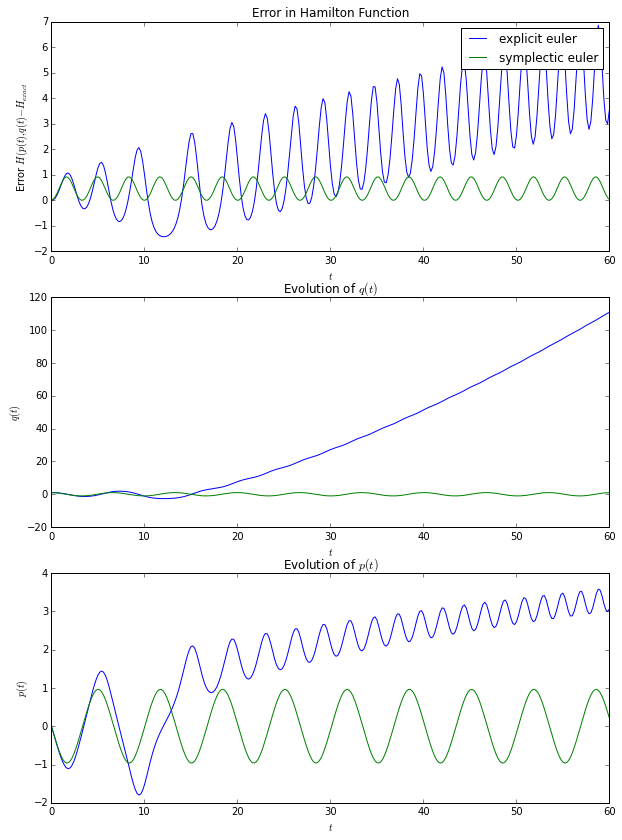
\includegraphics[scale=0.4]{hw3_p1.png}
\end{center}

~\\
It is clear that for explicit euler method, $H$ gradually grows with $t$ as well as $q(t)$, and finally the object will go to infinitely faraway. For symplectic method $H$ is bounded in a range, and the motion of the pendulum has a regular behavior. 
\end{proof} 
\noindent\rule{16cm}{0.4pt}
%///////////////////////////////////////////////////////////////////////

\begin{problem} Implement implicit Euler, implicit midpoint method and trapezoid method, compare their rates of convergence and execution time. 

\end{problem}
\begin{solution} We plot $\log(n)$ against $\log(error)$ to check the rate of convergence. Theoretically, for a method of order $k$, we expect to get a line with slope $-k$.

\begin{center}
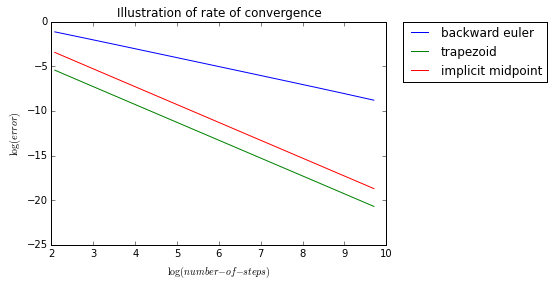
\includegraphics[scale=0.7]{hw3_p2.png}
\end{center}

~\\
Which is indeed the case. We see that backward euler converges in order 1, other 2 methods have order 2.

\begin{center}
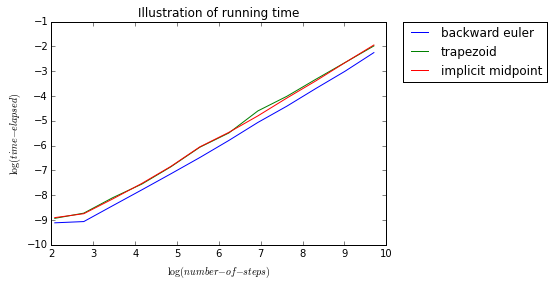
\includegraphics[scale=0.7]{hw3_p3.png}
\end{center}

~\\
We used the \emph{Secant Method} find roots for these implicit methods. The execution time are all $O(nm)$. Where $m$ is the average number of iterations it takes to find the zeros of implicit updating rules.

~\\
Finally we applied these methods to the testcase 5 in last homework. And plotted the numerical solution as below.

\begin{center}
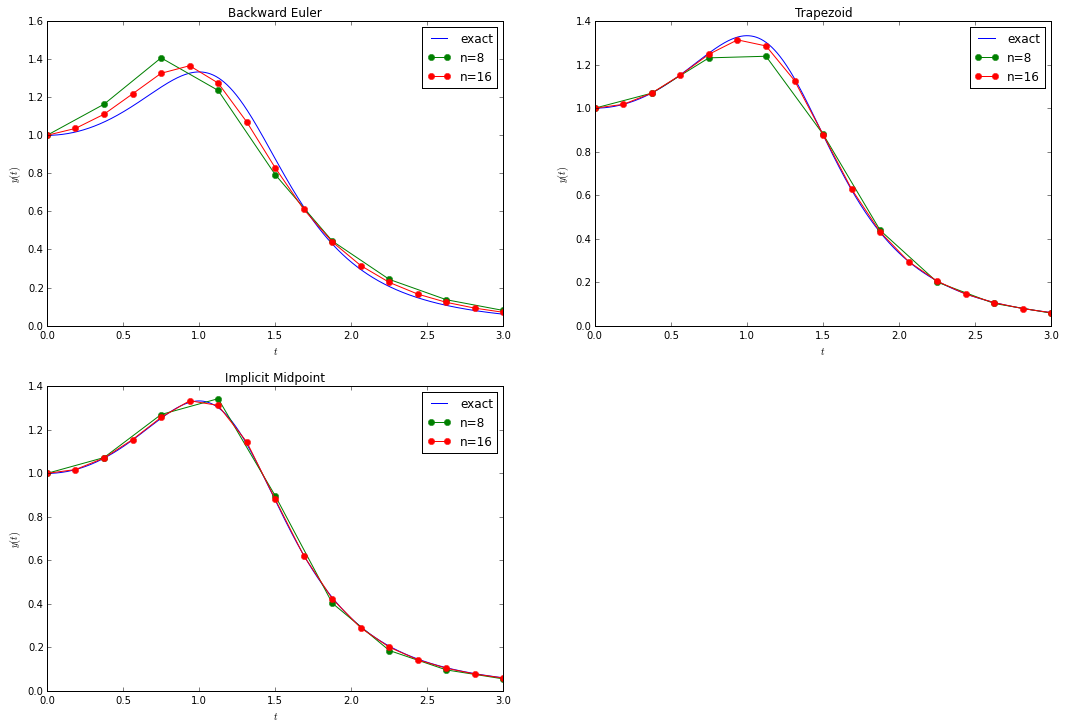
\includegraphics[scale=0.42]{hw3_p4.png}
\end{center}

~\\
Please also see the attached code for details.
\end{solution} 
\noindent\rule{16cm}{0.4pt}
%///////////////////////////////////////////////////////////////////////






\end{document}